\documentclass[10pt,twocolumn]{article}                                                                           
\renewcommand{\baselinestretch}{1.05}                                                                   
\usepackage{amsmath,amsthm,verbatim,amssymb,amsfonts,amscd, graphicx,listings,mathtools}                
\DeclarePairedDelimiter{\ceil}{\lceil}{\rceil}                                                          
\usepackage{graphics}                                                                                   
\usepackage{color}                                                                                      
\definecolor{mygreen}{rgb}{0,0.6,0}                                                                     
\definecolor{mygray}{rgb}{0.5,0.5,0.5}
\definecolor{mymauve}{rgb}{0.58,0,0.82}
\topmargin0.0cm
\headheight0.0cm
\headsep0.0cm
\oddsidemargin0.0cm
\textheight23.0cm
\textwidth16.5cm
\footskip1.0cm
\usepackage{listings}
\renewcommand{\thefigure}{\arabic{section}.\arabic{figure}} 
% \addtolength{\topmargin}{-1.0in}
\usepackage{ marvosym }
\usepackage{subcaption}
\usepackage{amsmath} 
\usepackage{hyperref}


% something NOT relevant to the usage of the package.


 \begin{document}
 % $insert math here$ and \[inset math here \] represent the math environment
 % within the math environment we have:
        % \; - a thick space
        % \: - a medium space
        % \, - a thin space
        % \! - a negative thin space
 % indentation only holds within listings.
\title{Spectral Clustering on Similarity Based networks}
\author{s1235260}
\maketitle 




\section{Abstract}
The aim of this mini project is to study the evolution of interest based spacial communities by exploiting the properties of the Laplacian matrix of a graph to carry out spectral clustering on communities with growing radii. 

% \newline

 To test these methods we will use real data extracted from the popular dating app Tinder which allows us to collect nodes (people) within a certain radius in addition to biographies which we will use to create edges in between people to symbolize that they may know each other.
\newline
% \newline
All together we will be using methods from machine learning (unsupervised), spectral graph theory, statistics and classical dynamics.

% \newline
The purpose of this project is exploratory and ideally the aim is to gain reasonable insights from spectral clustering on how the data evolves as we increase the radius.

\section{Physical Motivation}
In this section I aim to motivate the use of eigen vectors in spectral community detection by
taking of from interpreting the Laplacian as the second derivative operator $(\nabla \cdot \nabla) = \nabla^{2}$ :

First lets start of with a vector $\underline{u}(t)$
where each component $u_{i}(t)$ represents the amount of energy or heat in a node. Additional we allow edges to permit heat flow in between nodes thus if one attempts to model the evolution of the system (of $N$ nodes) with respect to determine the rate of $u_{i}(t)$  as the following:
\[
\frac{d}{dt}u_{i}(t) = -\kappa \sum_{j=1}^{N}A_{ij}(u_{i}(t) -u_{j}(t))
\]
Where :

\[ A_{ij} = \begin{cases} 
   1 \quad when \; i \text{ is coneccted to } j \\
   0 \quad otherwise 
   \end{cases}
\]

Which makes sense since this will yield the rate of change of $u_{i}(t)$ at one time step as the differences $u_{i}(t) - u_{j}(t)$ for all nodes $j$ connected to node $i$. This tells us how the rate of energy evolves in the system.
\newline
Distributing the sum operator:

\[
\frac{d}{dt}u_{i}(t) = -\kappa \left( u_{i}(t) \sum_{j=1}^{N}A_{ij}-  \sum_{j=1}^{N}A_{ij}u_{j}(t) \right )
\]
We know that if we sum up row 1 in matrix $A$ we find out the number of nodes incident on node 1 which we define as the degree of node 1. Generalizing this to $i$ follows trivially:

\[
\frac{d}{dt}u_{i}(t) = -\kappa \left( u_{i}(t) deg(i)-  \sum_{j=1}^{N}A_{ij}u_{j}(t) \right )
\]

Since $A_{ii}=0$  (A node connected to itself is trivial in our system and thus it is not accounted/allowed) we can use the kronecker delta symbol to rewrite this more compactly:

\[ \delta_{ij} = \begin{cases} 
   1 \quad when \; i = j \\
   0 \quad otherwise 
   \end{cases}
\]

\[
\frac{d}{dt}u_{i}(t) = -\kappa \sum_{j=1}^{N}(\delta_{ij} deg(i) -A_{ij}u_{j}(t))
\]
Which we can compact in to the vector matrix form (Where $D$ is the diagonal degree matrix):
\[
\frac{d}{dt}\underline{u}(t) = -\kappa\underbrace{(D -A)}_{L}\underline{u}(t)
\]
This gives us a first order linear system of differential equations (similar to the heat equation if $L = \nabla^{2}$). Due to basic properties of matrix algebra solving this equation is rather trivial. I will provide a run through solution given that we ignore initial conditions for simplicity.
\[
\frac{d}{dt}\underline{u}(t) = -\kappa L\underline{u}(t)
\]
Lets guess the following ansazt to this ODE (common method in physics) as $\underline{v}e^{-\kappa\lambda t}$ where $\underline{v}$ is some constant vector. Plugging in to the heat equation (and canceling out equal terms) we now have:

\[
 \lambda \underline{v} = L \underline{v}
\]

Which we recognize as a typical eigen value eigen vector equation. Which we can solve easily but the important thing I would like to comment on is what the solution means about our system. The different eigenvalues $\lambda$ (also known as the spectrum of $L$) describe how every different solution (mode) to our heat equation changes dynamically since our solutions are of the form :  $\underline{v}_{i}e^{-\kappa\lambda_{i} t}, \quad i \in N$ so bigger lambdas may imply that our system is experiencing a decaying transfer of energy in time the eigen vector itself also tells us about the dynamics of the energy transfer since each of its component represents a node and in contrast to the others it tells us how the coupled system is simultaneously transferring energy (i.e. One node giving the other loosing , energy transfer in sync etc..). Thus in a sense the eigen vectors by describing the different possible dynamics of energy transfer in the system tell us different things about connectivity in the graph and thus can  help us find elements that may be clique like meaning that they all like to be connected to each other like a clique of friends.

\section{Graph Construction}
The first step is to construct a graph $G_{Tinder}(V,E)$ over which we will be using our spectral methods to study how communities evolve. In order to connect two people together we look at their biographies and based on a similarity measure which will be developed in this chapter we decide if they know each other or not. 
\subsection{How Tinder Works}
Tinder is a mobile phone app which randomly pulls out people near by you (you define how near) and you swipe left or right depending if you like them or not. Most people include biographies and we also know the distance they are from you. So in this setting our phones are the origin of the ball of radius. Luckily for us we don't have to swipe since tinder has an API that allows us to  pull out as many people as we want using a simple python wrapper.
\subsection{Cosine Similarity Measure}
The cosine similarity measure for two vectors $\underline{v} $ and $\underline{u}$ (s.t. $\underline{v}, \underline{u} \in \mathbb{R}^{n}$) is defined as the following:
\[
cos(\theta) = \frac{\underline{v}\cdot \underline{u}}{||\underline{v}|| \: ||\underline{u}||}
\]
which just tells us how close two vectors are too each other. Now all we need to do this is transform our biographies in to vectors. In order to do this we check the words existing across all biographies and either make a word count vector or a binary vector for each node. Scikit learn provides us with a function to efficiently compute this. 
\newline\newline
Post to this
we can calculate the cosine similarity measure in between vectors which gives us a measure of how similar to bios are for all bios in our node space.
\newline\newline 
Now all we require to do is decide how to use this similarity measure to join nodes together. To do so we will make the assumption that most people dont have too much in common (low similarity coefficient) and the ones that have a lot in common are very likely to know each other. In the next sub chapter I will motivate and outline the mathematics behind this.
\subsection{Z-score Outlier test}
This is one of the most used statistical tests which has been widely popularized in particle physics when discovering a new particle. The idea behind this term is that very extreme values are likely to validate to contradict some null hypothesis which validates our original hypothesis. In our case we are going to use it to detect nodes that do not belong to the set of nodes that do not know each other.
\newline
To this we assume that our cosine similarity measures are normally distributed which as we can see by plotting a histogram of them they seem to be so:
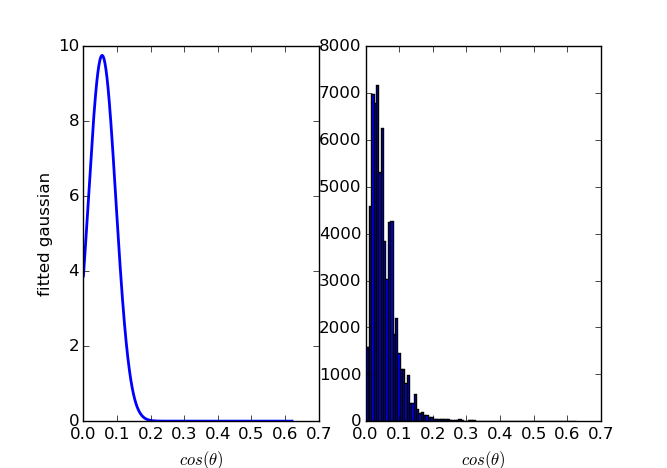
\includegraphics[scale=0.422]{pics/hist2.png}
As we can see the Gaussian fits rather nicely. The scale difference between the height of the Gaussian and histogram is due to the Gaussian being a pdf with a continuous range and thus its area elements are infinitesimally in $dx$ making it scale down.
\newline
Now given that our assumption seems reasonable we construct the following boolean test:
\[
(x_{\text{node pair coefficient}} - \mu) > 2\sigma
\]

Where: $$\mu = \frac{1}{N^{2}}\sum_{x \in \text{node coefficients pairs} } x$$  $$\sigma = \frac{1}{N^{2}}\sum_{x \in \text{node coefficients pairs} } (x- \mu)^{2}$$
What our boolean test tells us is that if a coefficient $x_{\text{node pair coefficient}}$ is away from the mean of our coefficient pair distribution by twice the standard deviation then it is 95\%  likely that this pair does not belong to this distribution of people that do not know each other and thus implying that they know each meaning that we construct an edge between the two nodes over which the coefficient was computed. This yields us graphs of the form:
\hspace*{-2cm}
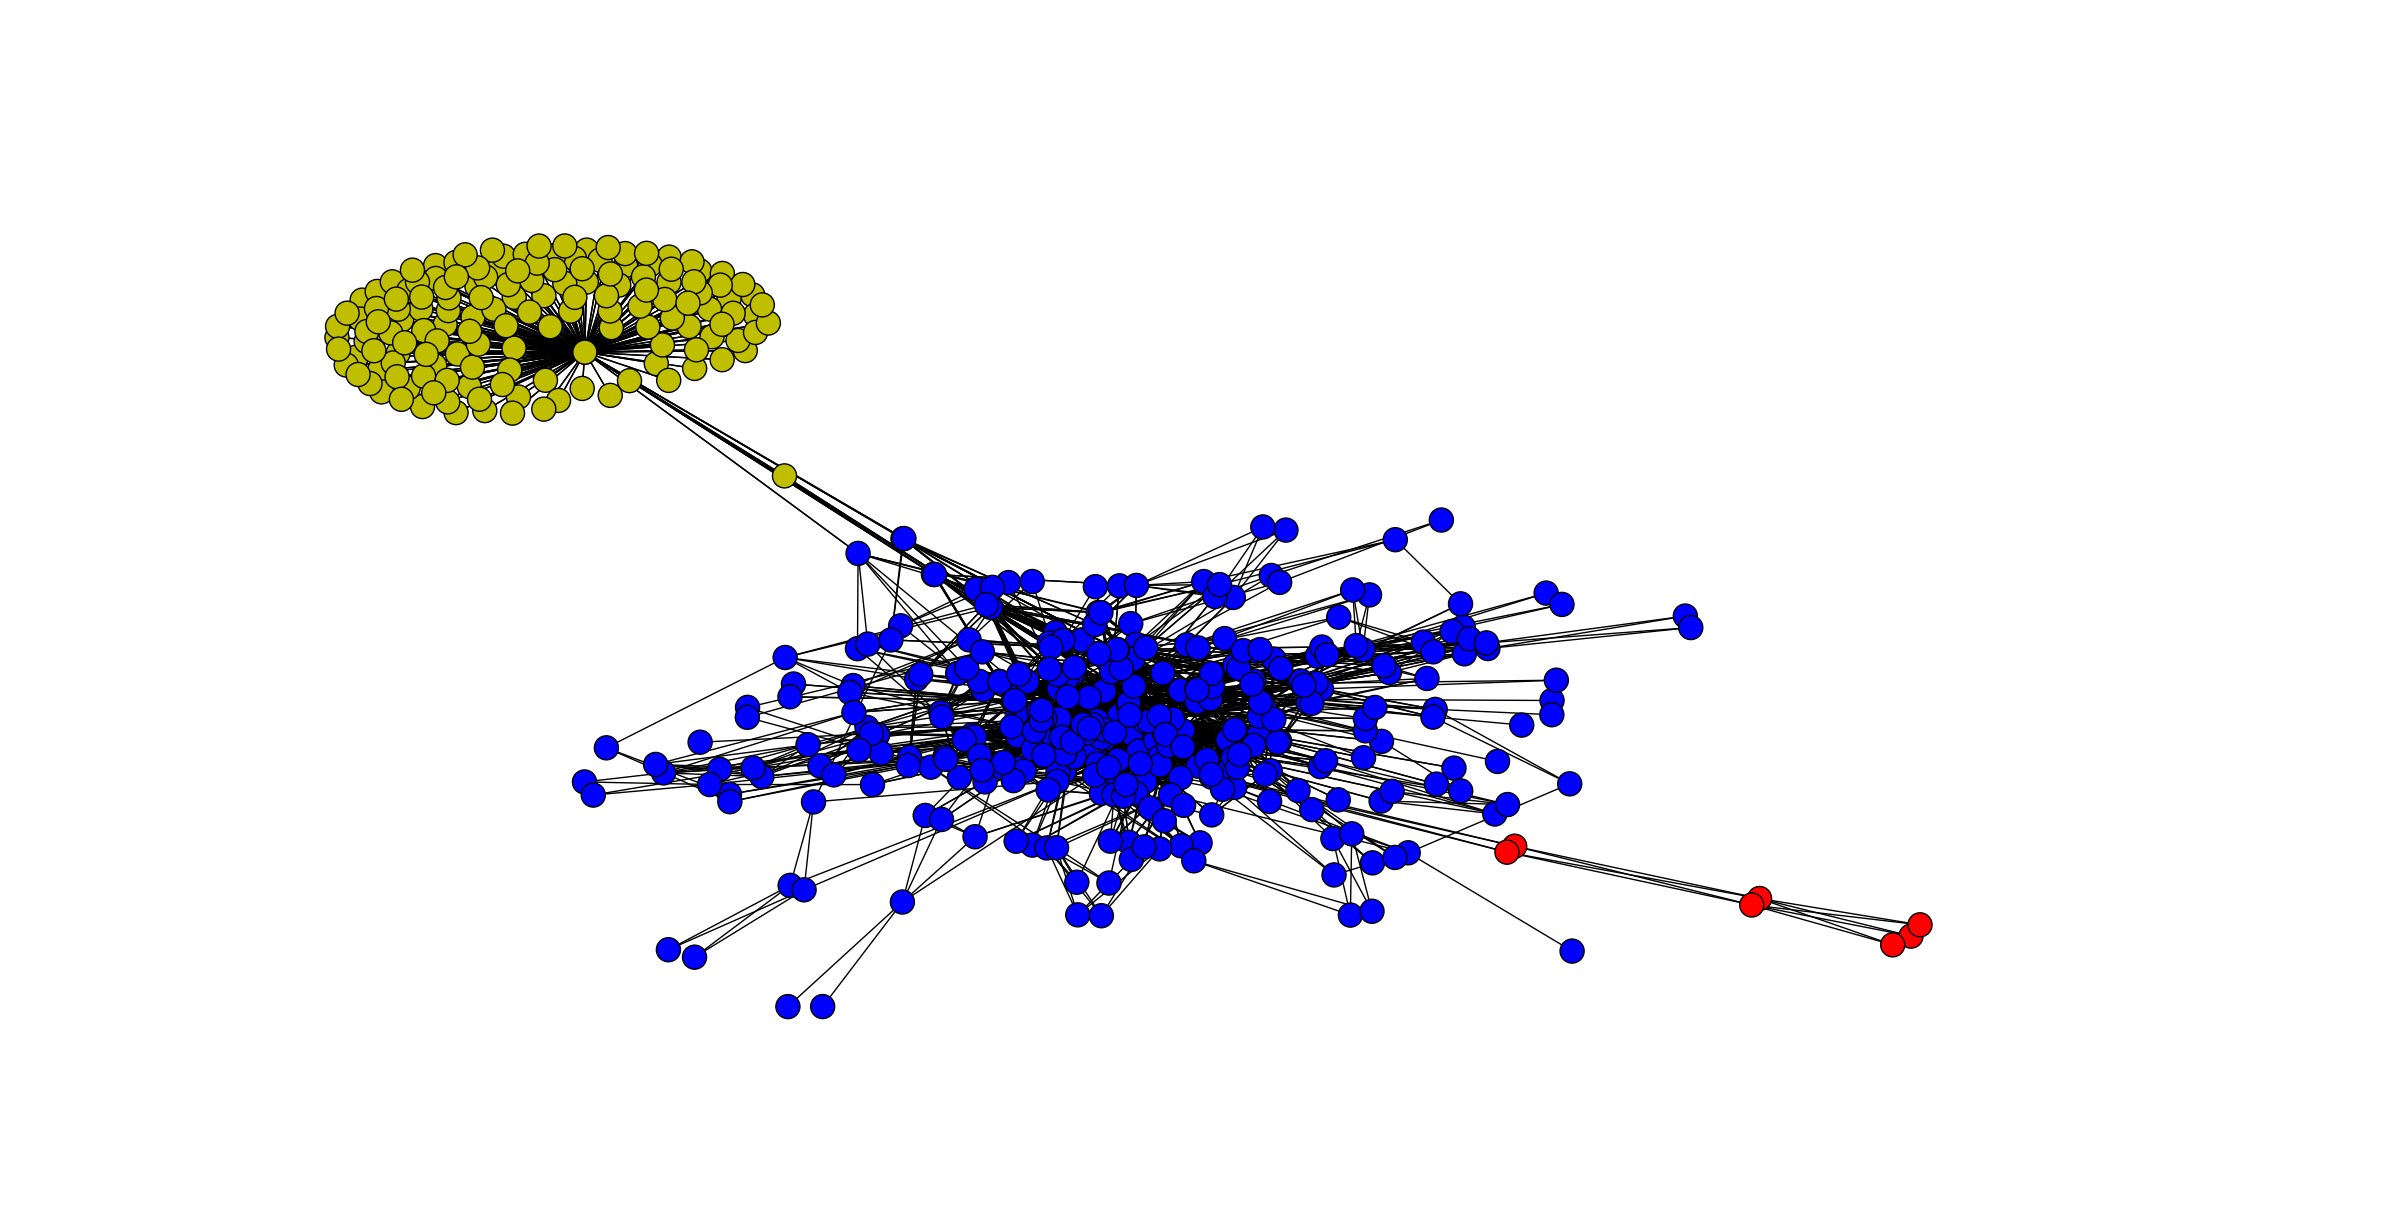
\includegraphics[scale=0.2]{pics/spring.png}
The colors are the result of our spectral clustering
for k=3 which we will discuss in the next chapter.
\section{Spectral Clustering}
As we have motivated previously clustering nodes by their Laplacian eigen space representation is a suitable idea for finding cliques and groups that are likely to know each other since in this space the nodes take values which describe connectivity properties over which it is useful to cluster.
\subsection{Algorithm Specification}
In pseudocode we can describe our spectral clustering algorithm as:
\begin{lstlisting}[mathescape]
$\mathcal{A}_{spectralClust}:$
$\textbf{Input } G(V,E), k$ for the number of clusters
$\textbf{Ouput } ClusteredNodes$
1.  L := Laplacian(G(V,E))
2.  $\Lambda$ := eigenValues(L)
3.  $V$ := eigenVectors(L) // $V's$ rows
                         // are eigen vectors
4.  $V$.sortInAscentBy($\Lambda$)
5   $V$ := fisrt k rows in $V$
6.  NodeKSpace := {}
7.  for $\underline{n_{k}}$ $\in$ $V^{T}$:
8.       NodeKSpace $U$ {$\underline{n_{k}}$}
9.  ClusteredNodes = kMeans(NodeKSpace, k)
\end{lstlisting}

Where we assume kMeans(NodeKSpace, k) to be a standard k-means clustering algorithm that returns points and the clusters they belong to in the same order as the input.  For k=2 in terms of eigen vectors 2 and 3 we get the following graph and cluster assignments:
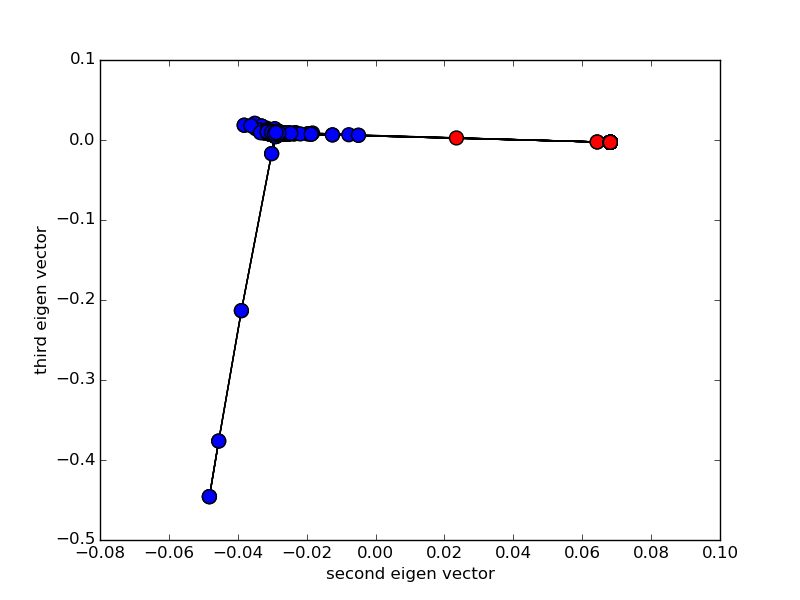
\includegraphics[scale=0.4]{pics/se.png}
With k=3:

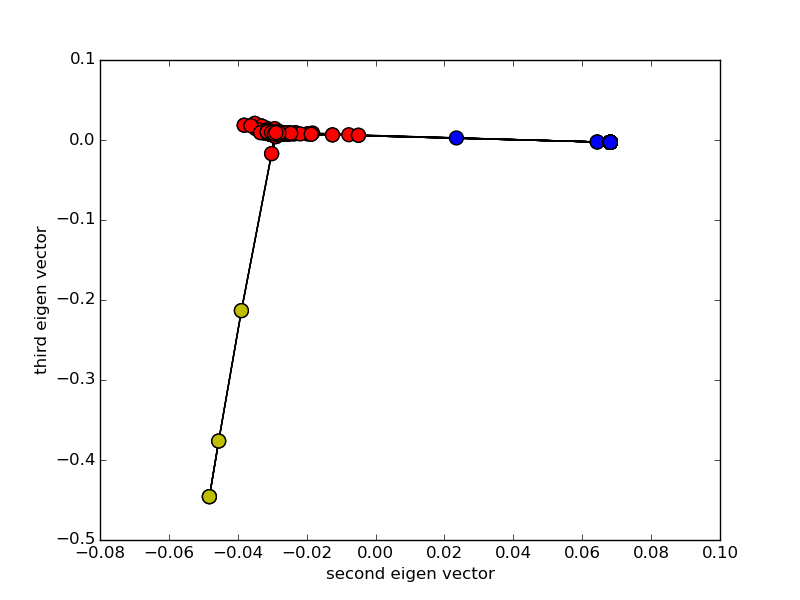
\includegraphics[scale=0.4]{pics/s.png}
\subsection{Picking the Number of Clusters}
In order to pick the number of clusters we used
the inter cluster aggregate  distance which is often used in machine learning to deal with this task:
\[
\sum_{c \in centroidSet} \sum_{\quad x \in c} D(x, c)^{2}
\]
Looking closely at this metric it gives us a sum of deviation distances about the centroid for each cluster. One can interpret it as an overall deviation metric as to how non dense (sparse) the clusters for a run of k-means are. Running this metric over different values of k ranging from 2 to 16 we get the following graph:
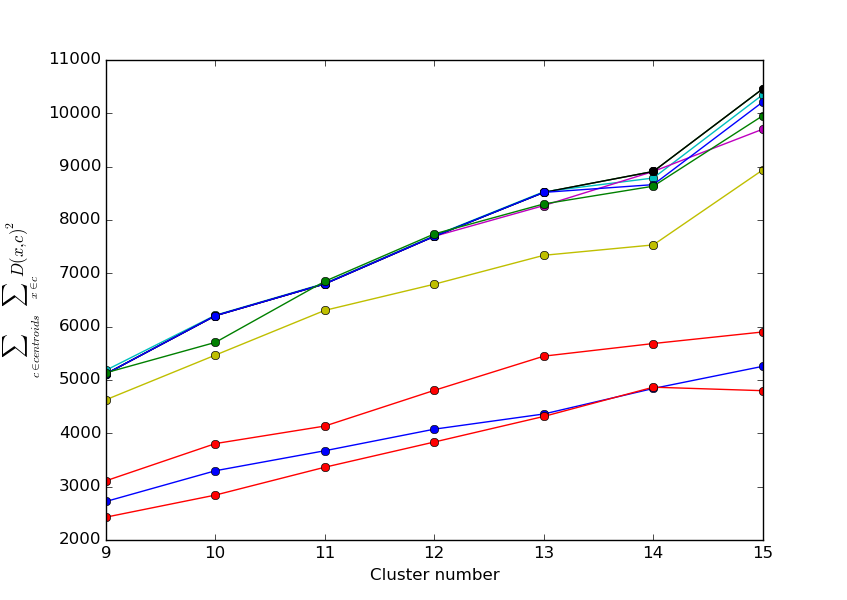
\includegraphics[scale=0.4]{pics/m.png}
We pick the number of clusters in such way to maxmise the the second derivative of this distance metric and by inspecting the graph we see the happens at 14 (the most accented change or the elbow looking pattern). We would normally expect this metric to go down with cluster number but since we increase the dimensionality of our nodes with k sparsity is also increased and thus making the metric go up.

\section{Community Evolution}

In this section we reach the end of our experiment
and it is where we asses how the communities (clusters) evolve as we increase the radius size allowing more people in Tinder to come in to our graph from further away locations.

\subsection{Dispersion of Radii}

As we did before in the cluster number picking
we will use the same metric to asses the density
of the communities as we grow the radius. This tells us how density of our communities changes
in space (radius). Which in a sense tells us how this aspect is evolving.
\newline\newline
We can explore our results (findings) by plotting the intra cluster aggregate distance vs the radii size (for our best cluster number 14):
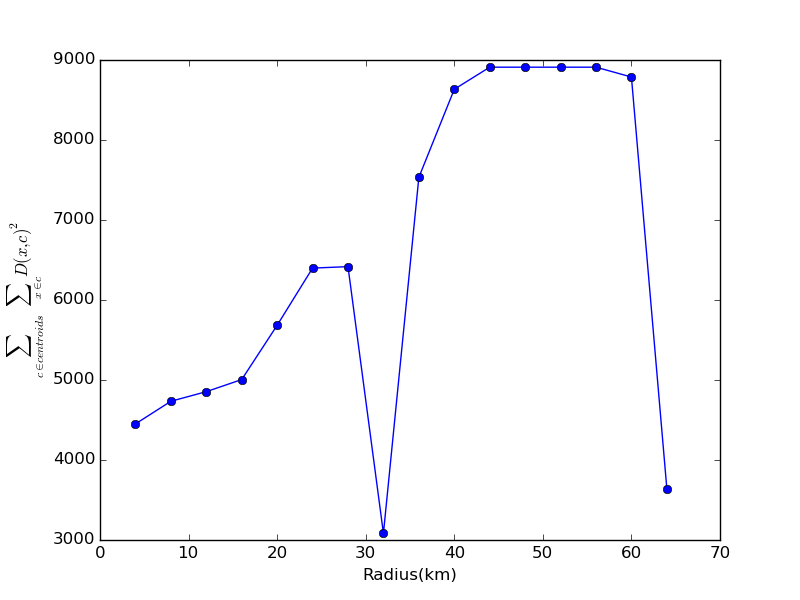
\includegraphics[scale=0.4]{pics/radii.png}

As we can observe the density of the clusters
seems to increase almost monotonically but then every now and then it experiences a decrease in density. 

I believe the partial monotonic increase is due to certain communities increasing  in density but after 30km it may be the case that we are getting closer to Glasgow or other towns in which the interest are very different to Edinburgh (Edinburgh being a cosmopolitan and international student city) and thus the new incomers are all quite far away from all the communities in Edinburgh but after we let the radius increase beyond this point the increase happens again.


I believe this increase is because these small isolated incomers are starting to form their own strong communities which shifts around the existing communities and may increase the densities of the new clusters.
\section{Bibliography}
\begin{enumerate}
% \usepackage{hyperref}
\item Einan Gardi , Dynamics \url{http://www2.ph.ed.ac.uk/~egardi/Dynamics/Dynamics_2014_lecture_12.pdf}
\item  Yale, Introduction to the Laplacian \url{http://www.cs.yale.edu/homes/spielman/561/2009/lect02-09.pdf}
\item V. Lavrenko, Clustering \url{http://www.inf.ed.ac.uk/teaching/courses/iaml/slides/kmeans-2x2.pdf}
\end{enumerate}
\end{document}
